\chapter{Methods}
\label{cha:methods}
This chapter contains the methods used for extending the existing hash based digital signature systems in this work.

\section{T5 Hashing}
Dodis et al.~\cite{T5_paper} propose a method called $T5$ for hashing five inputs with three hash compression calls. The $5n$-to-$n$ compression function $T5$ (with $n$ being the hash digest length) is constructed out of $2n$-to-$n$ compression functions $h_1, h_2, h_3$:

\begin{equation}
\label{eq:t5_basic}
T_5(m_1, m_2, m_3, m_4, m_5) = h_3(h_1(m_1,m_2) \oplus m_5, h_2(m_3,m_4) \oplus m_5) \oplus m_5
\end{equation}
It is proven by Dodis et al.~\cite{T5_paper} that the $T5$ construction matches Stam’s bound~\cite{stams_bound2008}, providing $\tilde{\mathcal{O}}(q^2/2^n)$ collision security and $\mathcal{O}(q^3/2^{2n}+nq/2^n)$, $q \leq 2^{n/2}$ preimage security. It provides birthday security $\mathcal{O}(2^{n/2})$ (see also Section~\ref{sec:omit_coll_res}) for hashing 5 inputs using three $2n$-to-$n$ compression calls, instead of only 4 inputs (in prior constructions). For the full proof of collision resistance and preimage resistance of $T5$, see Section~4.1 and Section~4.2 in~\cite{T5_paper}. % what is q not sure
Therefore, $T5$ is improving the Merkle-D\aa mgard construction (with the initialization vector counted as message block) and Merkle trees by processing a fifth message block with the same number of compression function calls and basically the same level of collision security. 
For this work, the construction of $T5$ in combination with Merkle trees is of interest.  

\subsection{T5 Block}
\label{sec:t5_block}
In Figure~\ref{img:t5_paper_block_depiction}, the construction of one \textit{T5-Block} out of a Merkle tree with height $d=2$ is shown:

\begin{itemize}
\item The variables  $m_1, m_2$ (respectively $m_3, m_4$) denote the left and right halves of input to compression function $h_1$ (respectively $h_2$).
\item The variable $a$ (respectively $b$) denotes the output of $h_1$ (respectively $h_2$).
\item The variables $c$ and $d$ denote the left and right halves of input to $h_3$.
\item The variable $e$ denotes the output of $h_3$.
\item The variable $f$ denotes the total output of $T5(m_1, m_2, m_3, m_4, m_5)$.
\end{itemize}
Therefore, the calculation of $T_5(m_1, m_2, m_3, m_4, m_5)$ consists of the following steps:
\begin{enumerate}
\item Calculation of the first layer of one $T_5$-Block (corresponds to compressing 4 leaves of a binary Merkle tree), two hash function calls $h_1, h_2$ are necessary:
\begin{align}
a = h_1(m_1, m_2) \\
b = h_2(m_3, m_4)
\end{align}

\item Calculation of the first $T_5$-specific intermediate step, adding $m_5$:
\begin{align}
c = a \oplus m_5 \\
d = b \oplus m_5
\end{align}

\item Calculation of the second layer of one $T_5$-Block (corresponds to compressing 2 nodes of a binary Merkle tree), one hash function calls $h_3$ is necessary:
\begin{align}
e = h_3(c,d)
\end{align}

\item Adding $m_5$ again (the second $T_5$ specific intermediate step) leads to the final result $f$:
\begin{align}
f = e \oplus m_5 = T_5(m_1, m_2, m_3, m_4, m_5)
\end{align}
\end{enumerate}

\begin{figure}
\centering
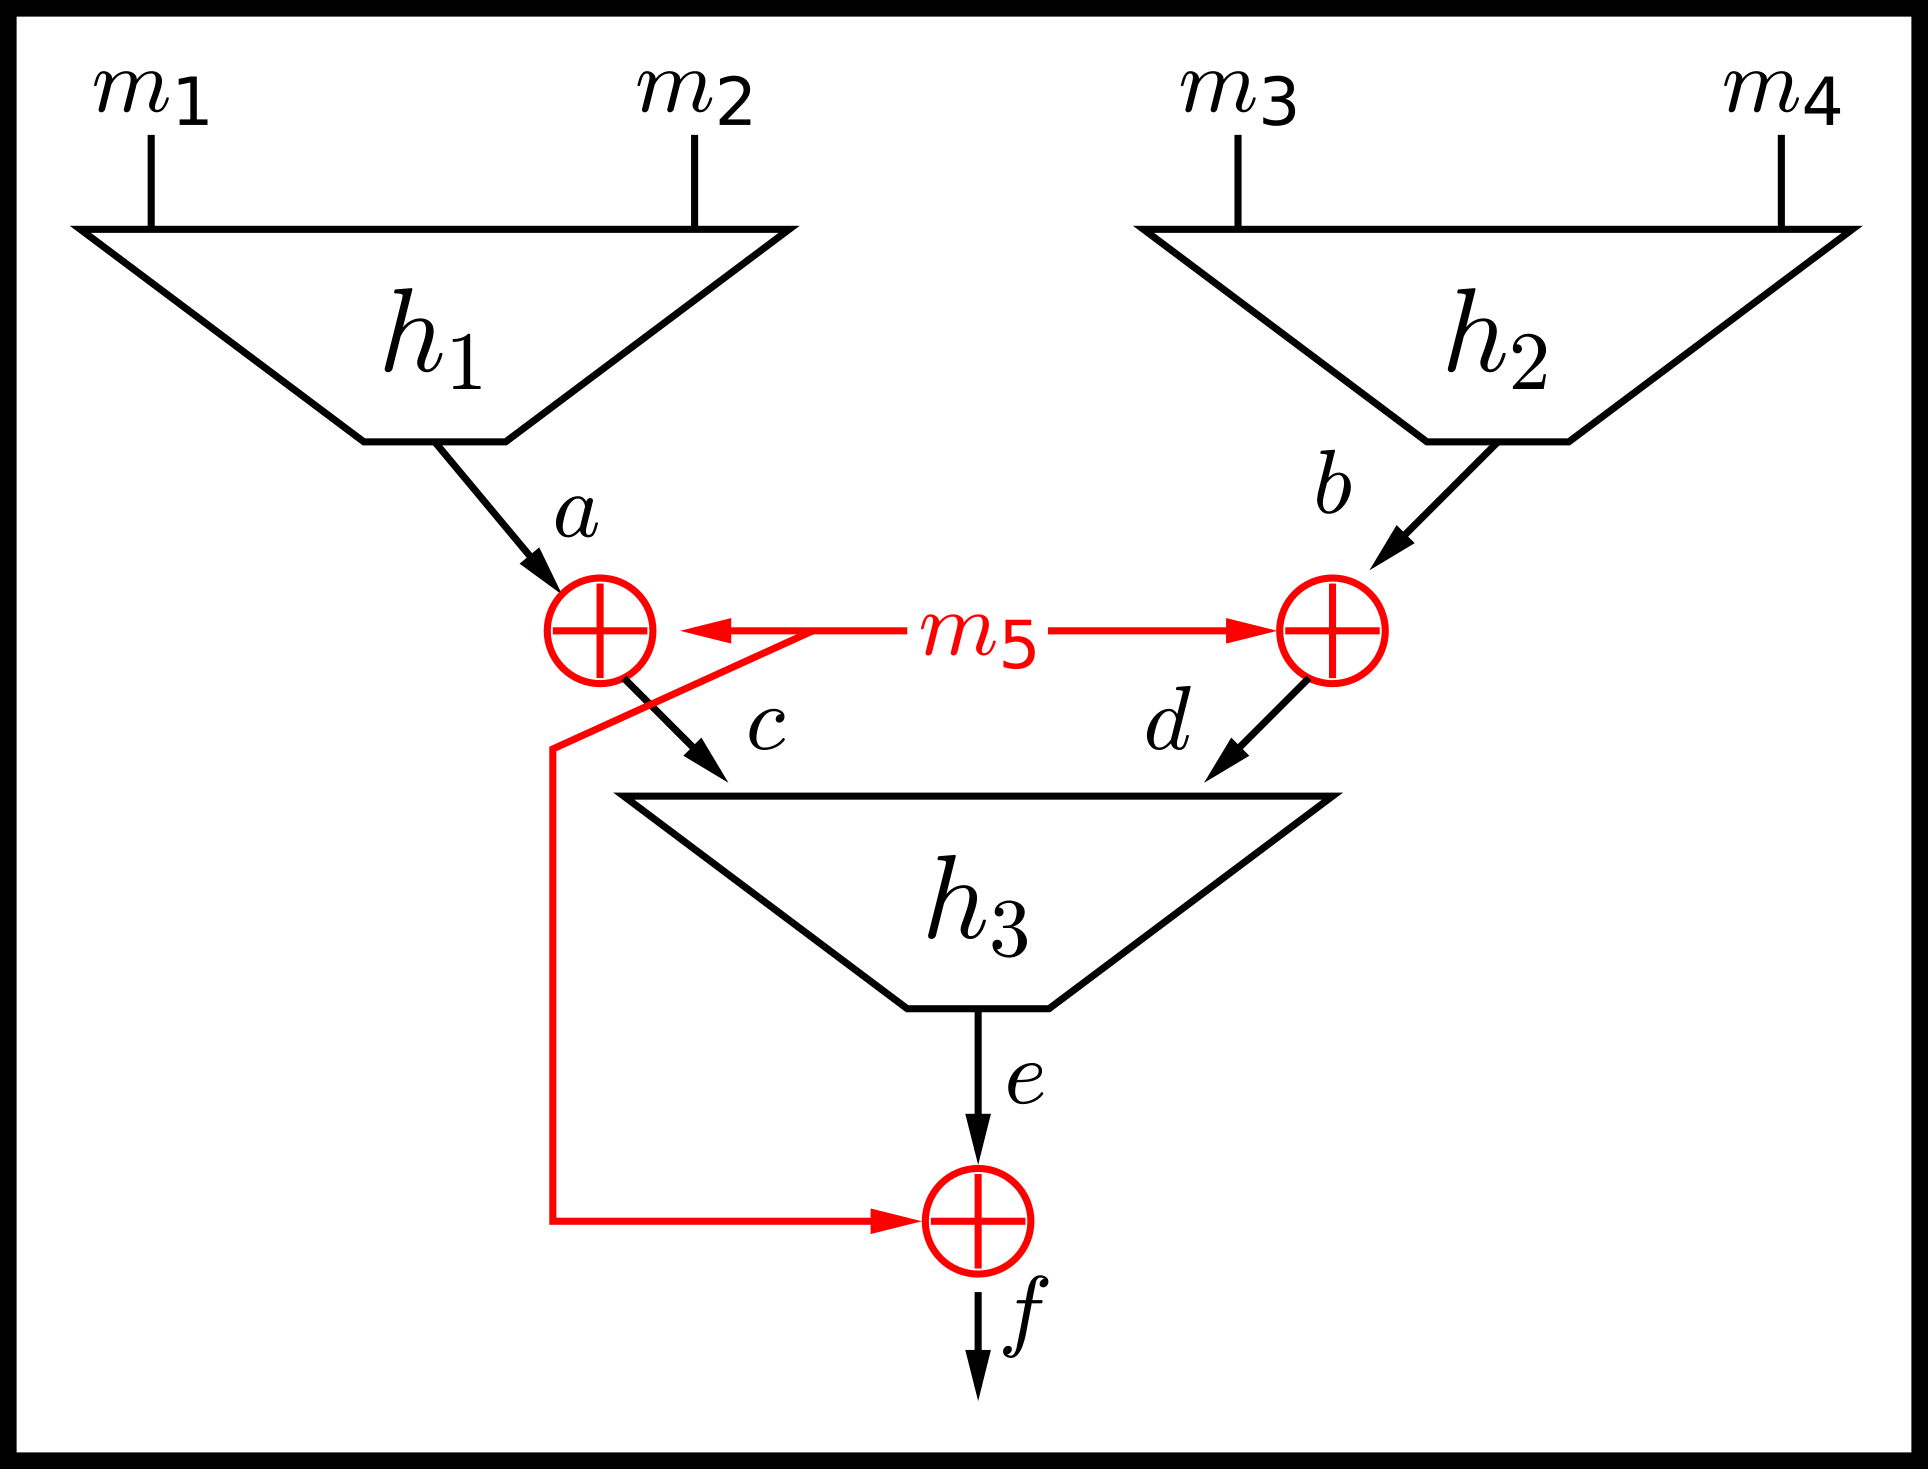
\includegraphics[]{images/Methods/abcd_paperT5_block_depiction.png}
\caption{Modified Merkle tree $T_5(m_1, m_2, m_3, m_4, m_5)$ of height d = 2,   with an extra input $m_5$ for the same 3 hash calls $h_1, h_2, h_3$. In this work, it is referred to as one $T_5$-Block.~\cite{T5_paper}}
\label{img:t5_paper_block_depiction}
\end{figure}

\subsection{T5 Openings}
To calculate the authentication path (see also Section~\ref{sec:mss_sig_gen} ) in one T5-Block, two different approaches \textit{Conservative Opening} and \textit{Aggressive Opening} are shown by Dodis et al.~\cite{T5_paper}. These two versions are depicted in Figure~\ref{img:t5_conserv_aggr_opening}.
The process of calculating an authentication path is here referred to as \textit{opening}. 

\subsubsection{Conservative Opening}
Given a node $m_i, i \in \{1,2,3,4\}$, the straightforward way to open the $T_5$-Block is to provide the remaining four nodes $m_{j \neq i}$. This is denoted as Conservative Opening and depicted in Figure~\ref{img:t5_conserv_aggr_opening}: The current node on the path is $m_1$ (colored green), the remaining four nodes (colored red) necessary for the authentication path to open $m_1$ are $m_2, m_3, m_4, m_5$. The functions $h_1, h_2, h_3$ (colored red) have to be calculated. The performance of the Conservative Method is less attractive than of the other methods and even worse than using a standard Merkle Tree: For authenticating one T5-Block, three hash calls and five elements in the authentication path are necessary, see also Table~\ref{table:conserv_opening}. Therefore, this method is not further considered in this work. % reference to authentication method with merkle tree -> #hashcalls, el. in authpath in table

\begin{table}
\centering
\begin{tabular}{l c} 
 \hline\noalign{\smallskip}
 \multicolumn{2}{c}{\textbf{Conservative Opening}} \\
 \hline\noalign{\smallskip}
 \# hashcalls & 3 \\
 \# el. in auth. path & 4 \\
 \hline
\end{tabular}
\caption{Performance of calculating the authentication path for one $T_5$-Block with Conservative Opening: The necessary amount of hashcalls and amount of elements in the authentication path are given.}
\label{table:conserv_opening}
\end{table}

\subsubsection{Aggressive Opening}
The second version of opening a $T_5$-Block with better performance than Conservative Opening is the Aggressive Opening. The provable security bounds decreases for this method, but the security remains the same under plausible attack scenarios. It is defined as follows: For a given opening node $m_i, i \in \{1,2,3,4,5\}$, the function $open_{auth}$ returns the authentication path elements for the corresponding $T_5$-Block:

\begin{align}
&open_{aggr}(m_1) = (m_2, m_5, h_2(m_3,m_4) \oplus m_5) = (m_2, m_5, d) \label{eq:aggr_open_m1_example} \\
&open_{aggr}(m_2) = (m_1, m_5, h_2(m_3,m_4) \oplus m_5) = (m_1, m_5, d) \\
&open_{aggr}(m_3) = (m_4, m_5, h_1(m_1, m_2) \oplus m_5) = (m_4, m_5, c) \\ 
&open_{aggr}(m_4) = (m_3, m_5, h_1(m_1, m_2) \oplus m_5) = (m_3, m_5, c) \\ 
&open_{aggr}(m_5) = (m_1, m_2, h_2(m_3, m_4) \oplus m_5) = (m_1, m_2, d) \label{eq:aggr_open_m5_example}
\end{align}
In Figure~\ref{img:t5_conserv_aggr_opening}, Aggressive Opening is depicted as example for opening node $m_1$ (colored green), see Equation~\ref{eq:aggr_open_m1_example}. 
As shown for all opening nodes in Equations~\ref{eq:aggr_open_m1_example}-\ref{eq:aggr_open_m5_example}, with the Aggressive Opening method the authentication path always contains three elements and the verifier needs two hash calls ($h_1$ or $h_2$ respectively and always $h_3$) to calculate the "root" $f$ of one $T_5$-Block, see Table~\ref{table:aggr_opening}.

\begin{table}
\centering
\begin{tabular}{l c} 
 \hline\noalign{\smallskip}
 \multicolumn{2}{c}{\textbf{Aggressive Opening}} \\
 \hline\noalign{\smallskip}
 \# hashcalls & 2 \\
 \# el. in auth. path & 3 \\
 \hline
\end{tabular}
\caption{Performance of calculating the authentication path for one $T_5$-Block with Aggressive Opening.}
\label{table:aggr_opening}
\end{table}

\begin{figure}
\centering
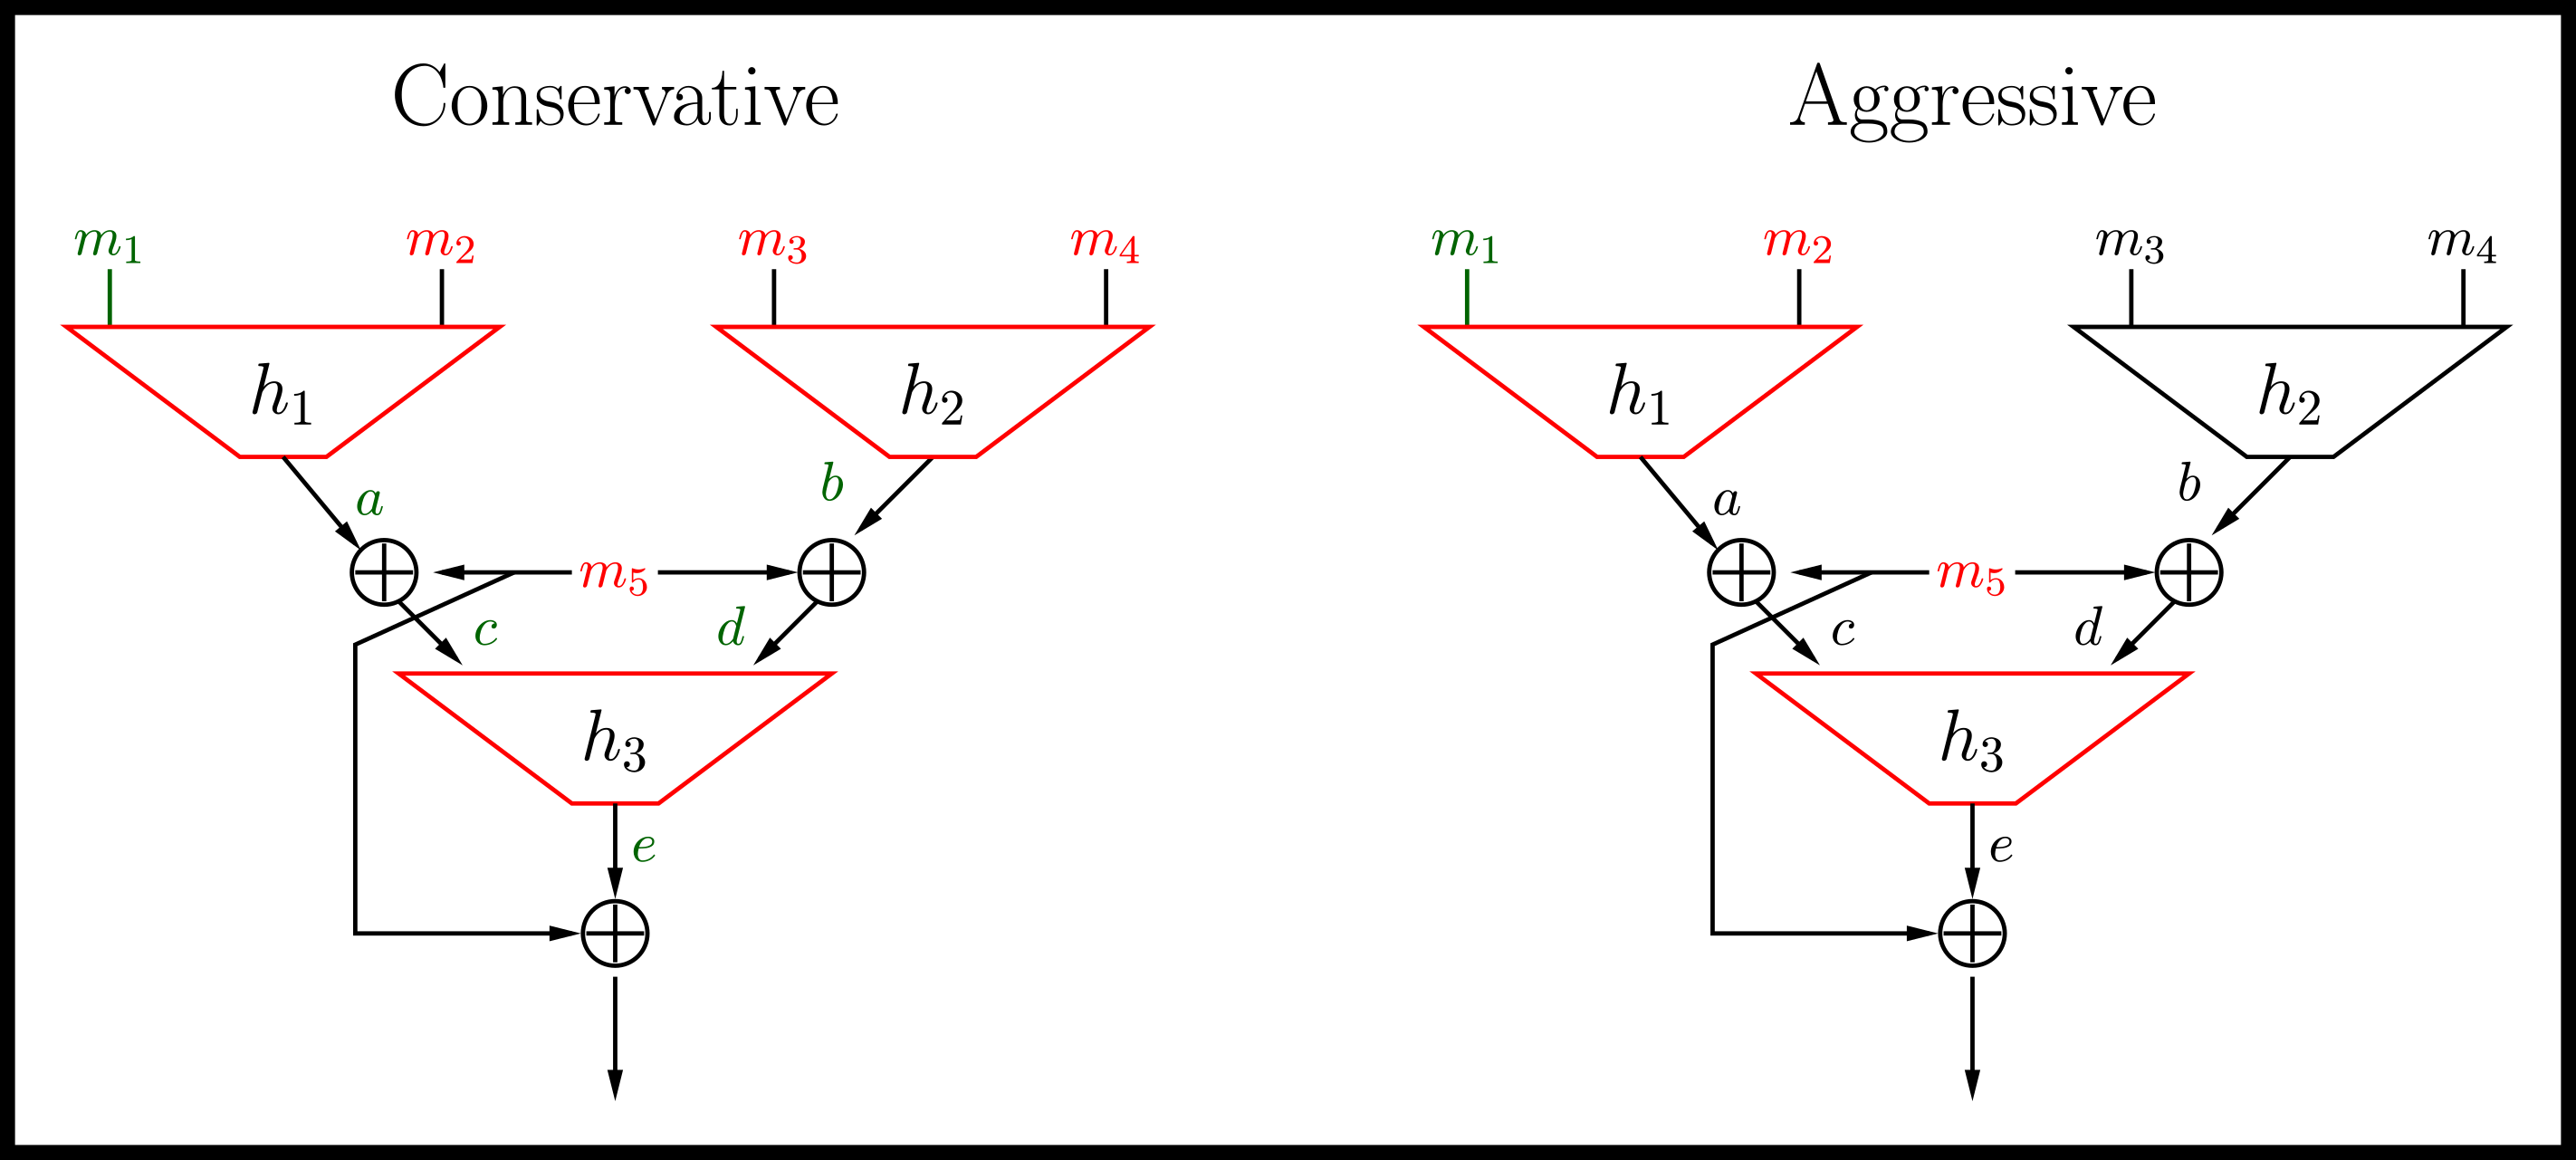
\includegraphics[]{images/Methods/aggr_conserv_opening_T5.png}
\caption{Conservative and Aggressive Opening of one $T_5$-Block. The green variable denotes the opening node, the red nodes are given in the authentication path for this $T_5$-Block. The hash functions denoted in red have to be calculated by the verifier to get the path for this $T_5$-Block.~\cite{T5_paper}}
\label{img:t5_conserv_aggr_opening}
\end{figure}

\subsection{T5 Merkle Tree}
Given the $T_5$-Block construction in Section~\ref{sec:t5_block}, a complete \textit{$T_5$ Merkle Tree} can be built. This is also shown by Dodis et al.~\cite{T5_paper}, see Figure~\ref{img:t5_complete_tree_paper}. Notably, the compression functions $h_1, h_2, h_3$ are the same function, the different indices are used for readability. The performance of the $T_5$ Merkle Tree (including Conservative- and Aggressive Opening variants) in comparison to the standard Merkle Tree is shown in Table~\ref{table:t5_merkletree_dodis_performance}: \textit{Build calls} denote the amount of hash calls necessary for building the whole $T_5$ Merkle Tree, \textit{opening} denotes thee length of the authentication path, \textit{verify} denotes the amount of hash calls needed to build the path (out of the authentication path). \textit{Tree depth} is the amount of layers in the binary Merkle tree compared with the amount of layers in $T_5$ Merkle tree - this corresponds to the amount of $T_5$ blocks $\times 2$ because one $T_5$ Block corresponds to two Merkle tree layers (see also Figure~\ref{img:t5_paper_block_depiction}).

\begin{table}
\centering
\begin{tabular}{l c c c} 
 \hline\noalign{\smallskip}
 \multicolumn{4}{c}{\textbf{$T_5$ Merkle Tree Performance}} \\
 \hline\noalign{\smallskip}
 & Merkle Tree (standard) & Conserv. Opening &  Aggr. Opening \\
 \hline\noalign{\smallskip}
 build calls$/t$ & 1 & 0.75 & 0.75 \\
 tree depth$/\log_2(t)$ & 1 & 0.86 & 0.86 \\
 verify (hash calls)$/\log_2(t)$ & 1 & 1.29 & 0.86 \\
 opening (length)$/\log_2(t)$ & 1 & 1.72 & 1.29 \\ 
 \hline
\end{tabular}
\caption{Performance of the $T_5$ Merkle Tree with the opening variants Conservative- and Aggressive Opening in comparison to the standard Merkle Tree given by Dodis et al.~\cite{T5_paper}. The variable $t$ denotes the amount of children.}
\label{table:t5_merkletree_dodis_performance}
\end{table}

\begin{figure}
\centering
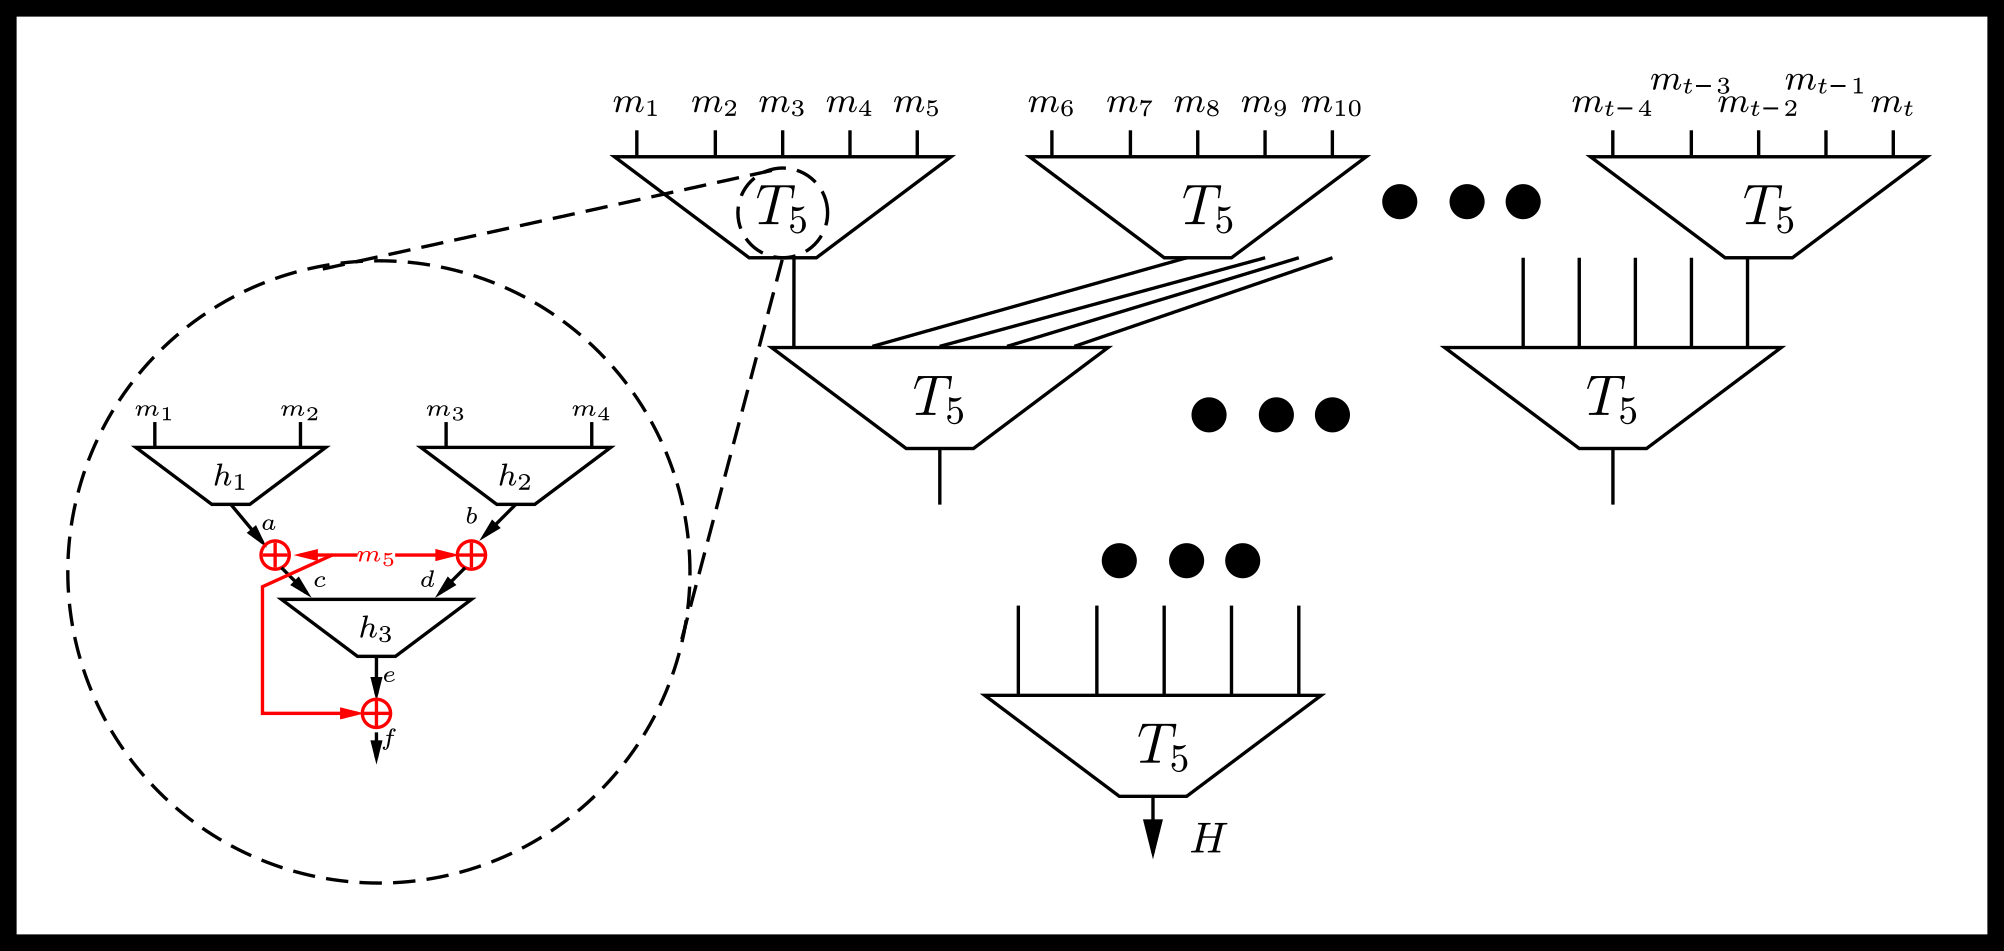
\includegraphics[]{images/Methods/whole_tree_T5_paper.png}
\caption{Construction of a complete $T_5$-Tree consisting of several $T_5$-Blocks~\cite{T5_paper}. The value $H$ denotes the root of the tree.}
\label{img:t5_complete_tree_paper}
\end{figure}

\section{Extended T5 Merkle Tree} % "my idea"
In this section, the idea of the $T_5$ Merkle tree is extended by an opening method \textit{More Aggressive Opening}, and the performance is compared to the \textit{Aggressive Opening} of Dodis et al.~\cite{T5_paper}. There is also a python implementation of the extended $T_5$ Merkle tree as digital signature scheme that contains the steps from key generation to signature verification, see Appendix~\ref{cha:appendix_t5_tree_implementation}.

\subsection{More Aggressive Opening}